\documentclass[12pt,ngerman,a4paperpaper,]{article}
\usepackage{lmodern}
\usepackage{amssymb,amsmath}
\usepackage{ifxetex,ifluatex}
\usepackage{fixltx2e} % provides \textsubscript
\ifnum 0\ifxetex 1\fi\ifluatex 1\fi=0 % if pdftex
  \usepackage[T1]{fontenc}
  \usepackage[utf8]{inputenc}
\else % if luatex or xelatex
  \ifxetex
    \usepackage{mathspec}
  \else
    \usepackage{fontspec}
  \fi
  \defaultfontfeatures{Ligatures=TeX,Scale=MatchLowercase}
\fi
% use upquote if available, for straight quotes in verbatim environments
\IfFileExists{upquote.sty}{\usepackage{upquote}}{}
% use microtype if available
\IfFileExists{microtype.sty}{%
\usepackage{microtype}
\UseMicrotypeSet[protrusion]{basicmath} % disable protrusion for tt fonts
}{}
\usepackage[unicode=true]{hyperref}
\hypersetup{
            pdfborder={0 0 0},
            breaklinks=true}
\urlstyle{same}  % don't use monospace font for urls
\ifnum 0\ifxetex 1\fi\ifluatex 1\fi=0 % if pdftex
  \usepackage[shorthands=off,main=ngerman]{babel}
\else
  \usepackage{polyglossia}
  \setmainlanguage[]{german}
\fi
\usepackage{graphicx,grffile}
\makeatletter
\def\maxwidth{\ifdim\Gin@nat@width>\linewidth\linewidth\else\Gin@nat@width\fi}
\def\maxheight{\ifdim\Gin@nat@height>\textheight\textheight\else\Gin@nat@height\fi}
\makeatother
% Scale images if necessary, so that they will not overflow the page
% margins by default, and it is still possible to overwrite the defaults
% using explicit options in \includegraphics[width, height, ...]{}
\setkeys{Gin}{width=\maxwidth,height=\maxheight,keepaspectratio}
\IfFileExists{parskip.sty}{%
\usepackage{parskip}
}{% else
\setlength{\parindent}{0pt}
\setlength{\parskip}{6pt plus 2pt minus 1pt}
}
\setlength{\emergencystretch}{3em}  % prevent overfull lines
\providecommand{\tightlist}{%
  \setlength{\itemsep}{0pt}\setlength{\parskip}{0pt}}
\setcounter{secnumdepth}{0}
% Redefines (sub)paragraphs to behave more like sections
\ifx\paragraph\undefined\else
\let\oldparagraph\paragraph
\renewcommand{\paragraph}[1]{\oldparagraph{#1}\mbox{}}
\fi
\ifx\subparagraph\undefined\else
\let\oldsubparagraph\subparagraph
\renewcommand{\subparagraph}[1]{\oldsubparagraph{#1}\mbox{}}
\fi

% set default figure placement to htbp
\makeatletter
\def\fps@figure{htbp}
\makeatother

\usepackage{amsmath}
\usepackage{fancyhdr}
\usepackage{ dsfont }
\usepackage{blindtext}

\usepackage{multicol}
%\usepackage[top=1cm,left=0.8cm,bottom=1.5cm,right=0.8cm]{geometry}
\usepackage[left=3cm,right=3cm, bottom=2cm, top=2cm]{geometry}
\usepackage{setspace}
\setstretch{1}

\newcommand{\columnsbegin}{\begin{multicols}{2}}
\newcommand{\columnsend}{\end{multicols}}
\usepackage{pdfpages}

\date{}

\begin{document}

\subsection{Aufgabe 3}\label{aufgabe-3}

\subsubsection{Prozess}\label{prozess}

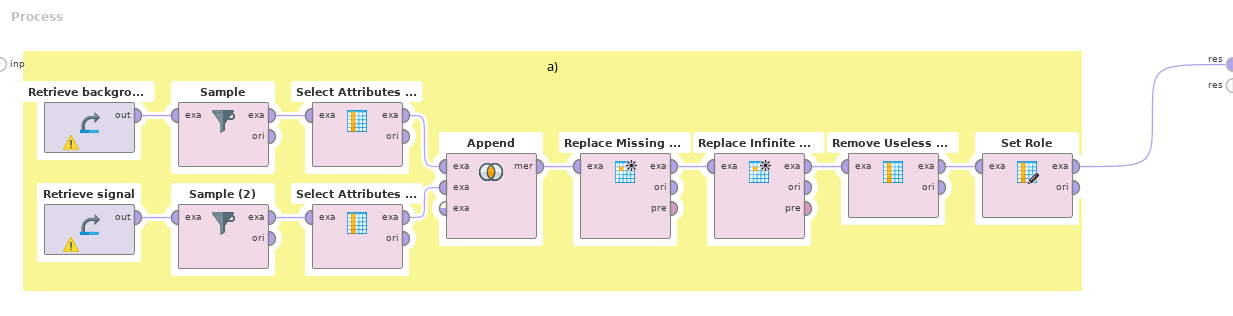
\includegraphics{aufg3/a.png} 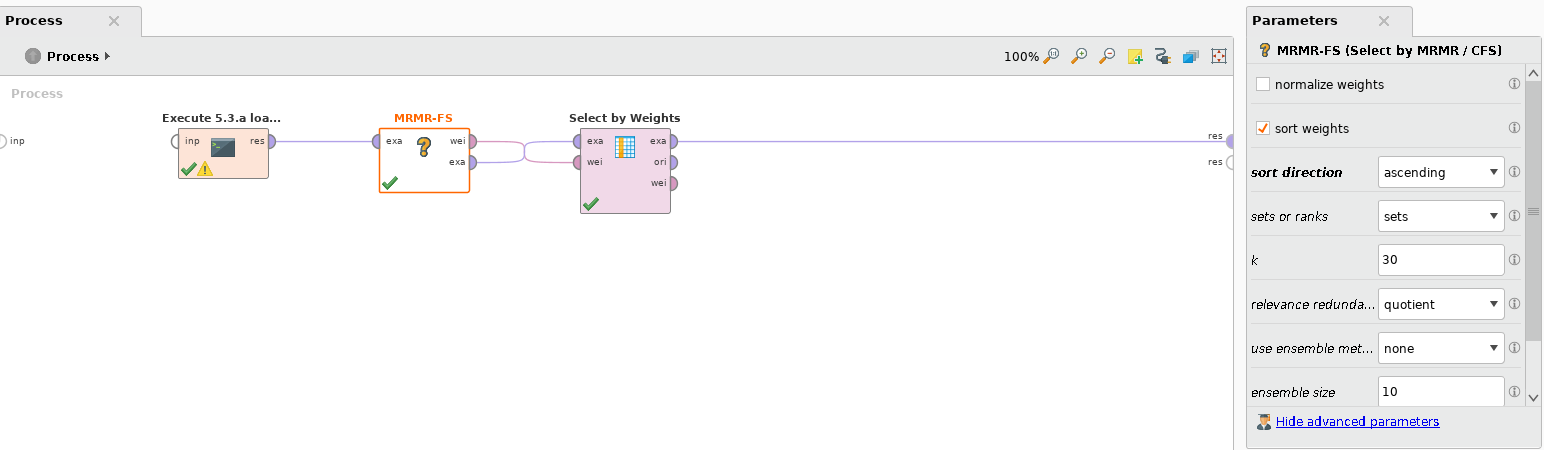
\includegraphics{aufg3/b.png}
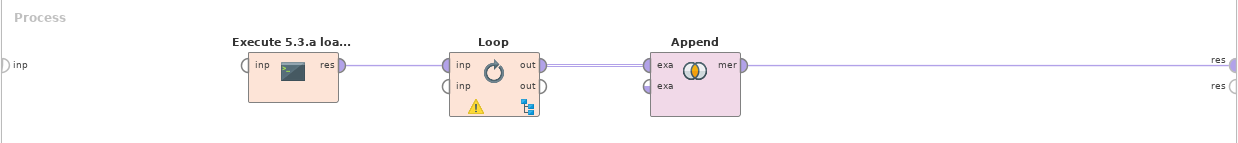
\includegraphics{aufg3/c1.png} 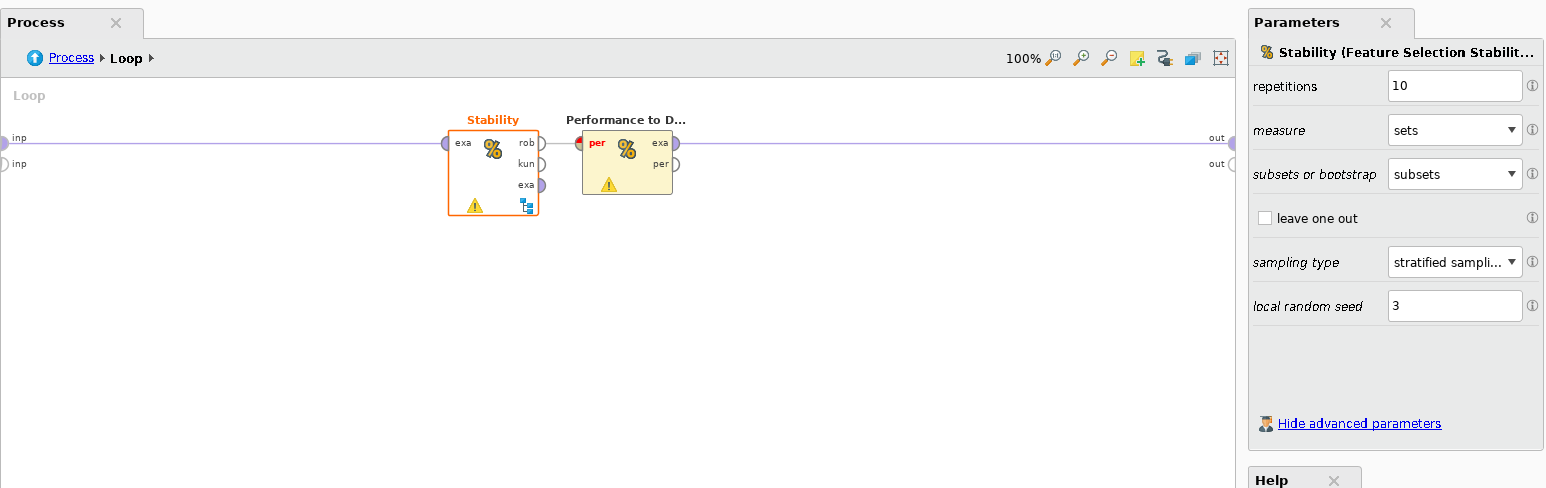
\includegraphics{aufg3/c2.png}
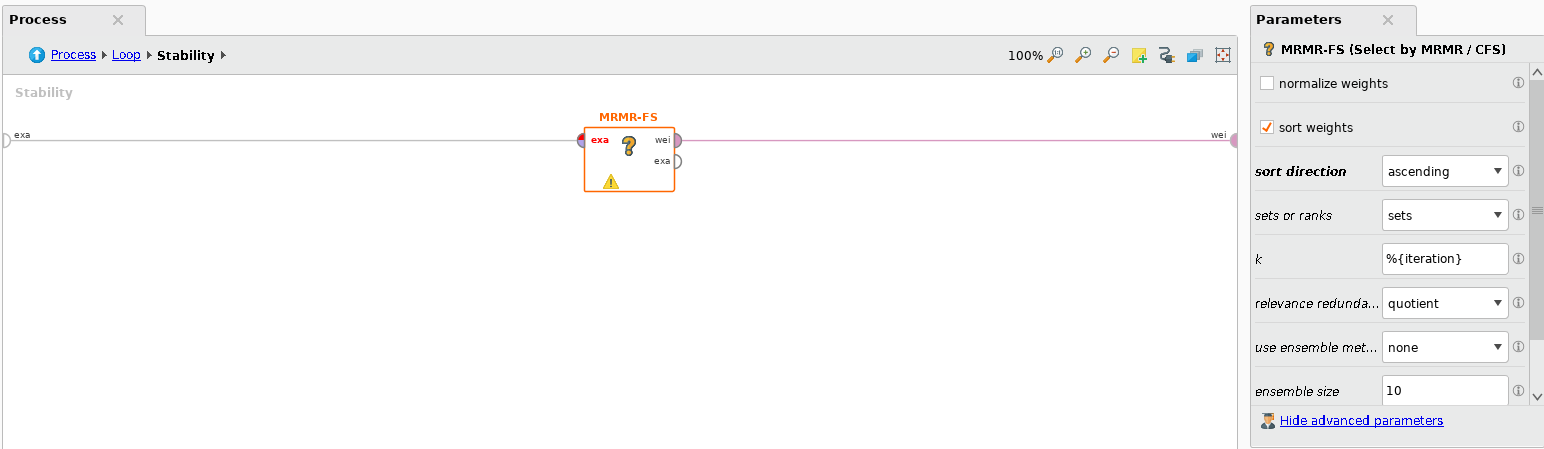
\includegraphics{aufg3/c3.png}

\subsubsection{Ergebnisse}\label{ergebnisse}

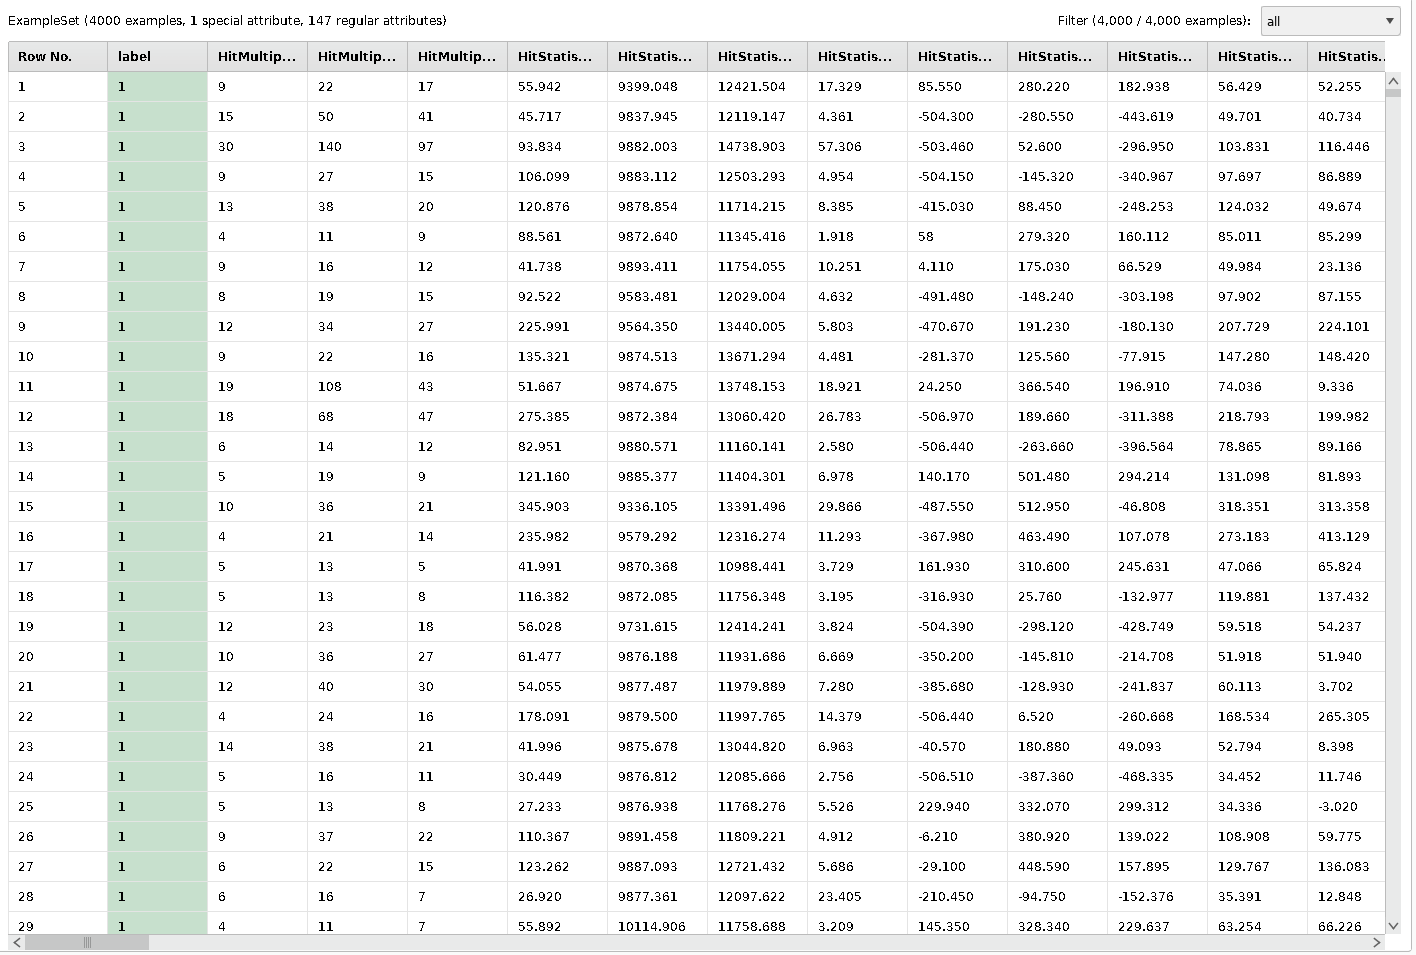
\includegraphics{aufg3/results-a.png}
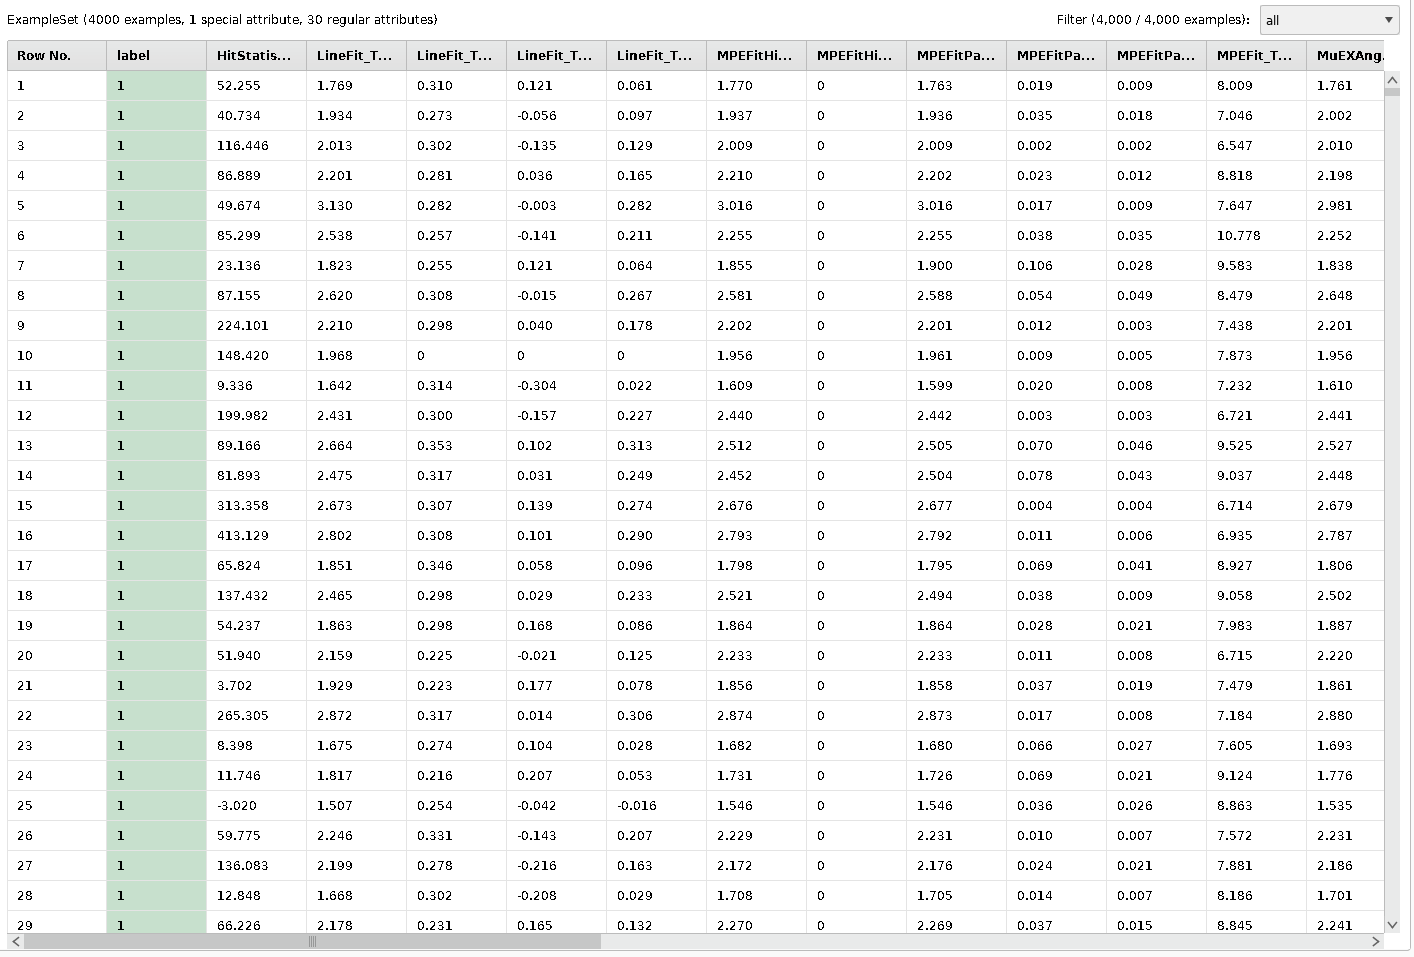
\includegraphics{aufg3/results-b.png}
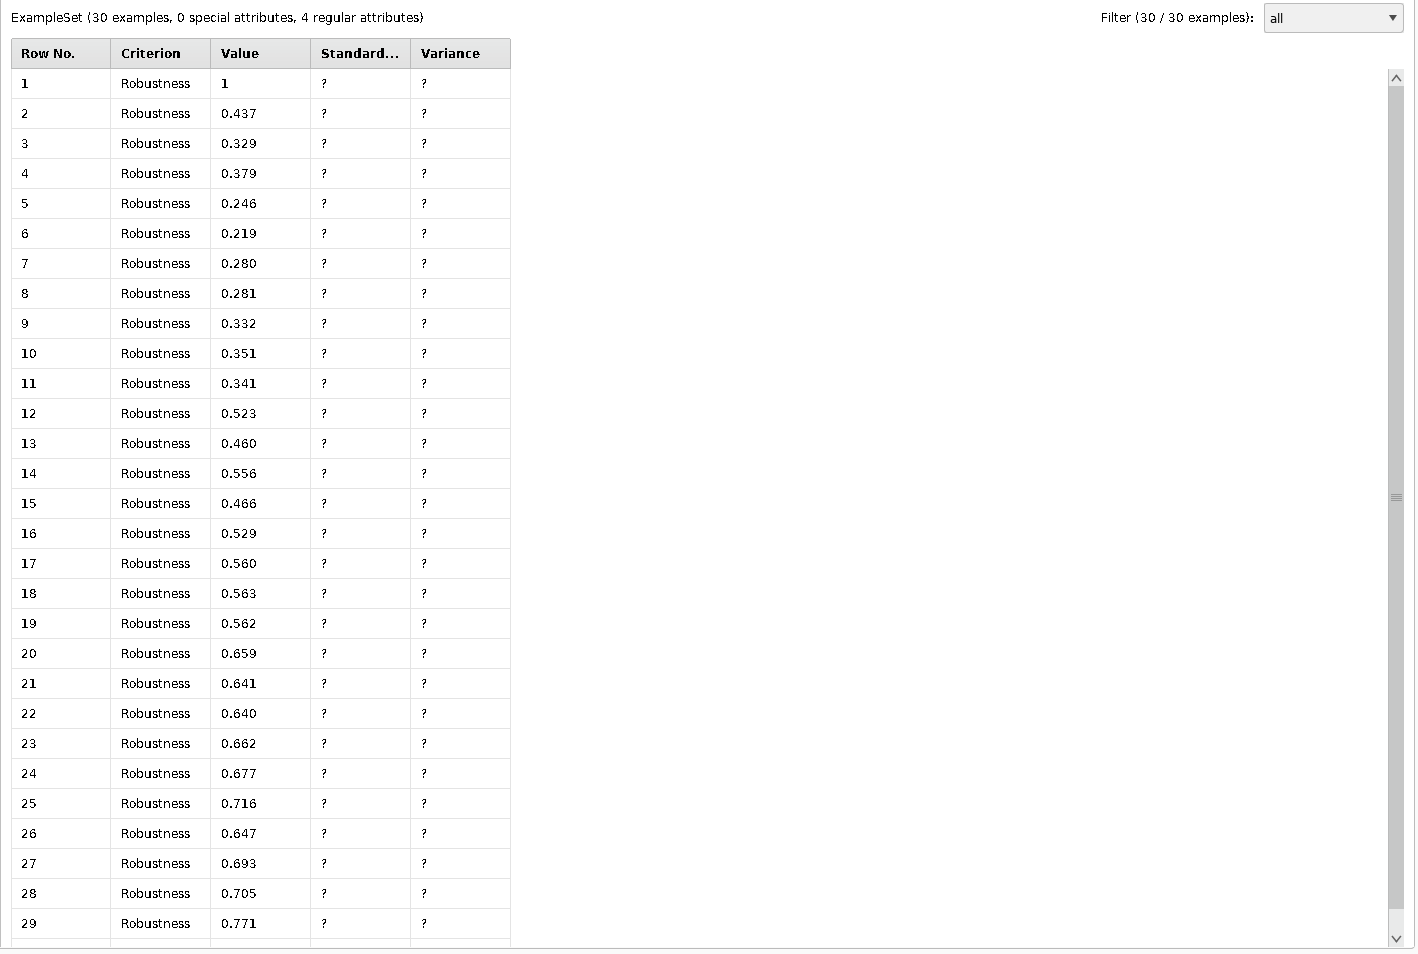
\includegraphics{aufg3/results-c.png}

\subsubsection{Robustheit}\label{robustheit}

\begin{figure}
\centering
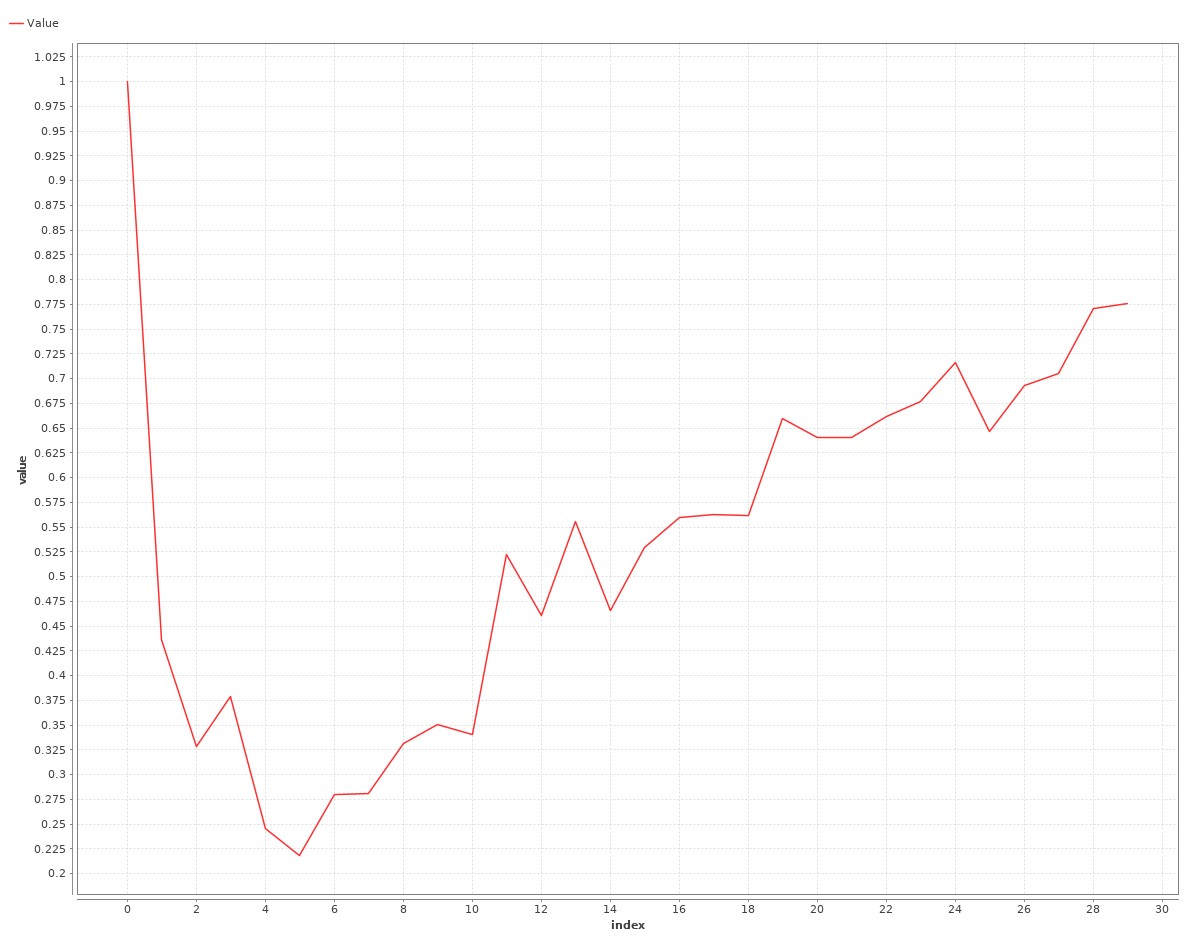
\includegraphics{aufg3/robustness.png}
\caption{Robustheit der MRMR Feature Selection für verschiedene Anzahl von Parametern.}
\end{figure}

Bei 0 Parametern ist die Unterscheidung zwischen Untgergrund und Signal
immer stabil (es gibt ja nur das Label). Ab dem Minimum bei 5 wird die
\emph{feature selection} immer stabiler, wie zu erwarten war (ein
Attribut `auf der Kippe' beeinflusst die Stabilität immer weniger, je
mehr Attribute es gibt).\\
Scheinbar ist die Wahl von weniger als 6 Attributen sehr instabil. Wie
viele Attribute man für das spezifische Problem behalten sollte hängt
von der Weiterverarbeitung ab; mehr sind jedoch (für \textgreater{}5
Attribute) tendenziell stabiler.

\end{document}
